%%%%
% -- Instrument Description
% --     FOBOS Keck White Paper 2019
%%%%


%%%%%%%%%%%%%%%%%%%%%%%%%%%%%%%%%%%%%%%%%%%%%%%%%%%%%%%%%%%%%%%%%%%%%%%%
\begin{figure}[h!]
%\vskip -0.1in
%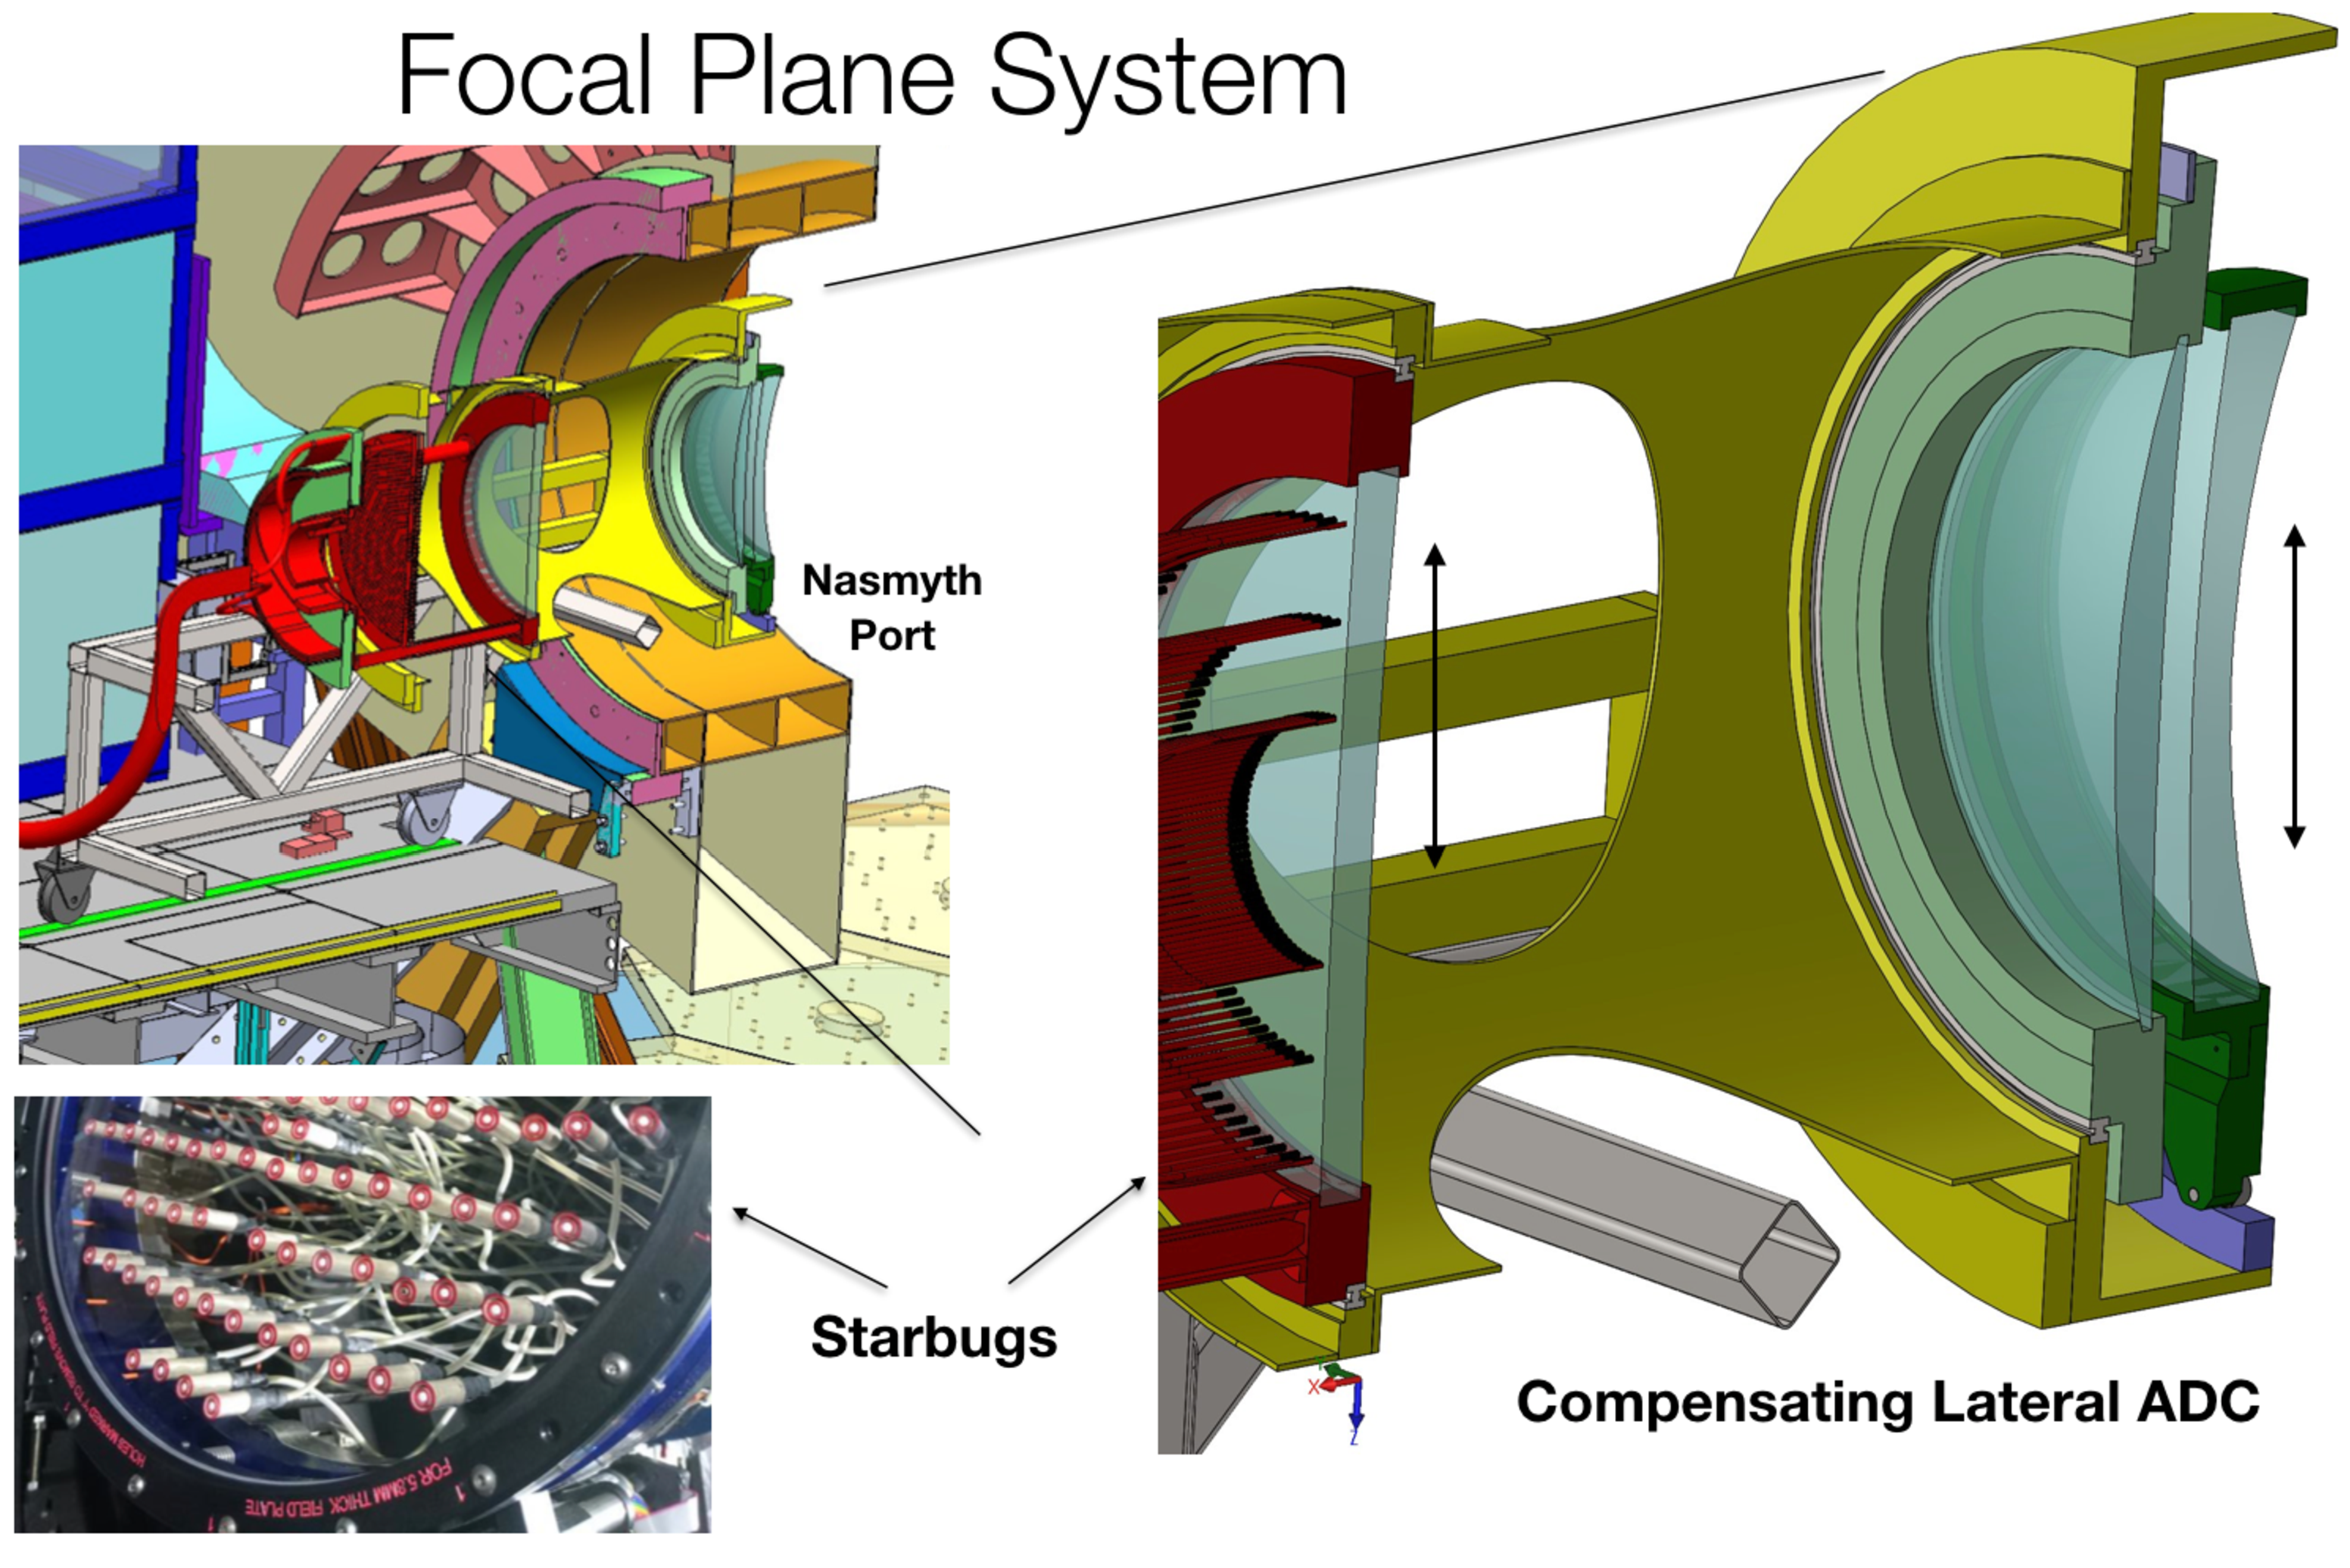
\includegraphics[width=\textwidth]{figs/FOBOS_FocalPlane.pdf}
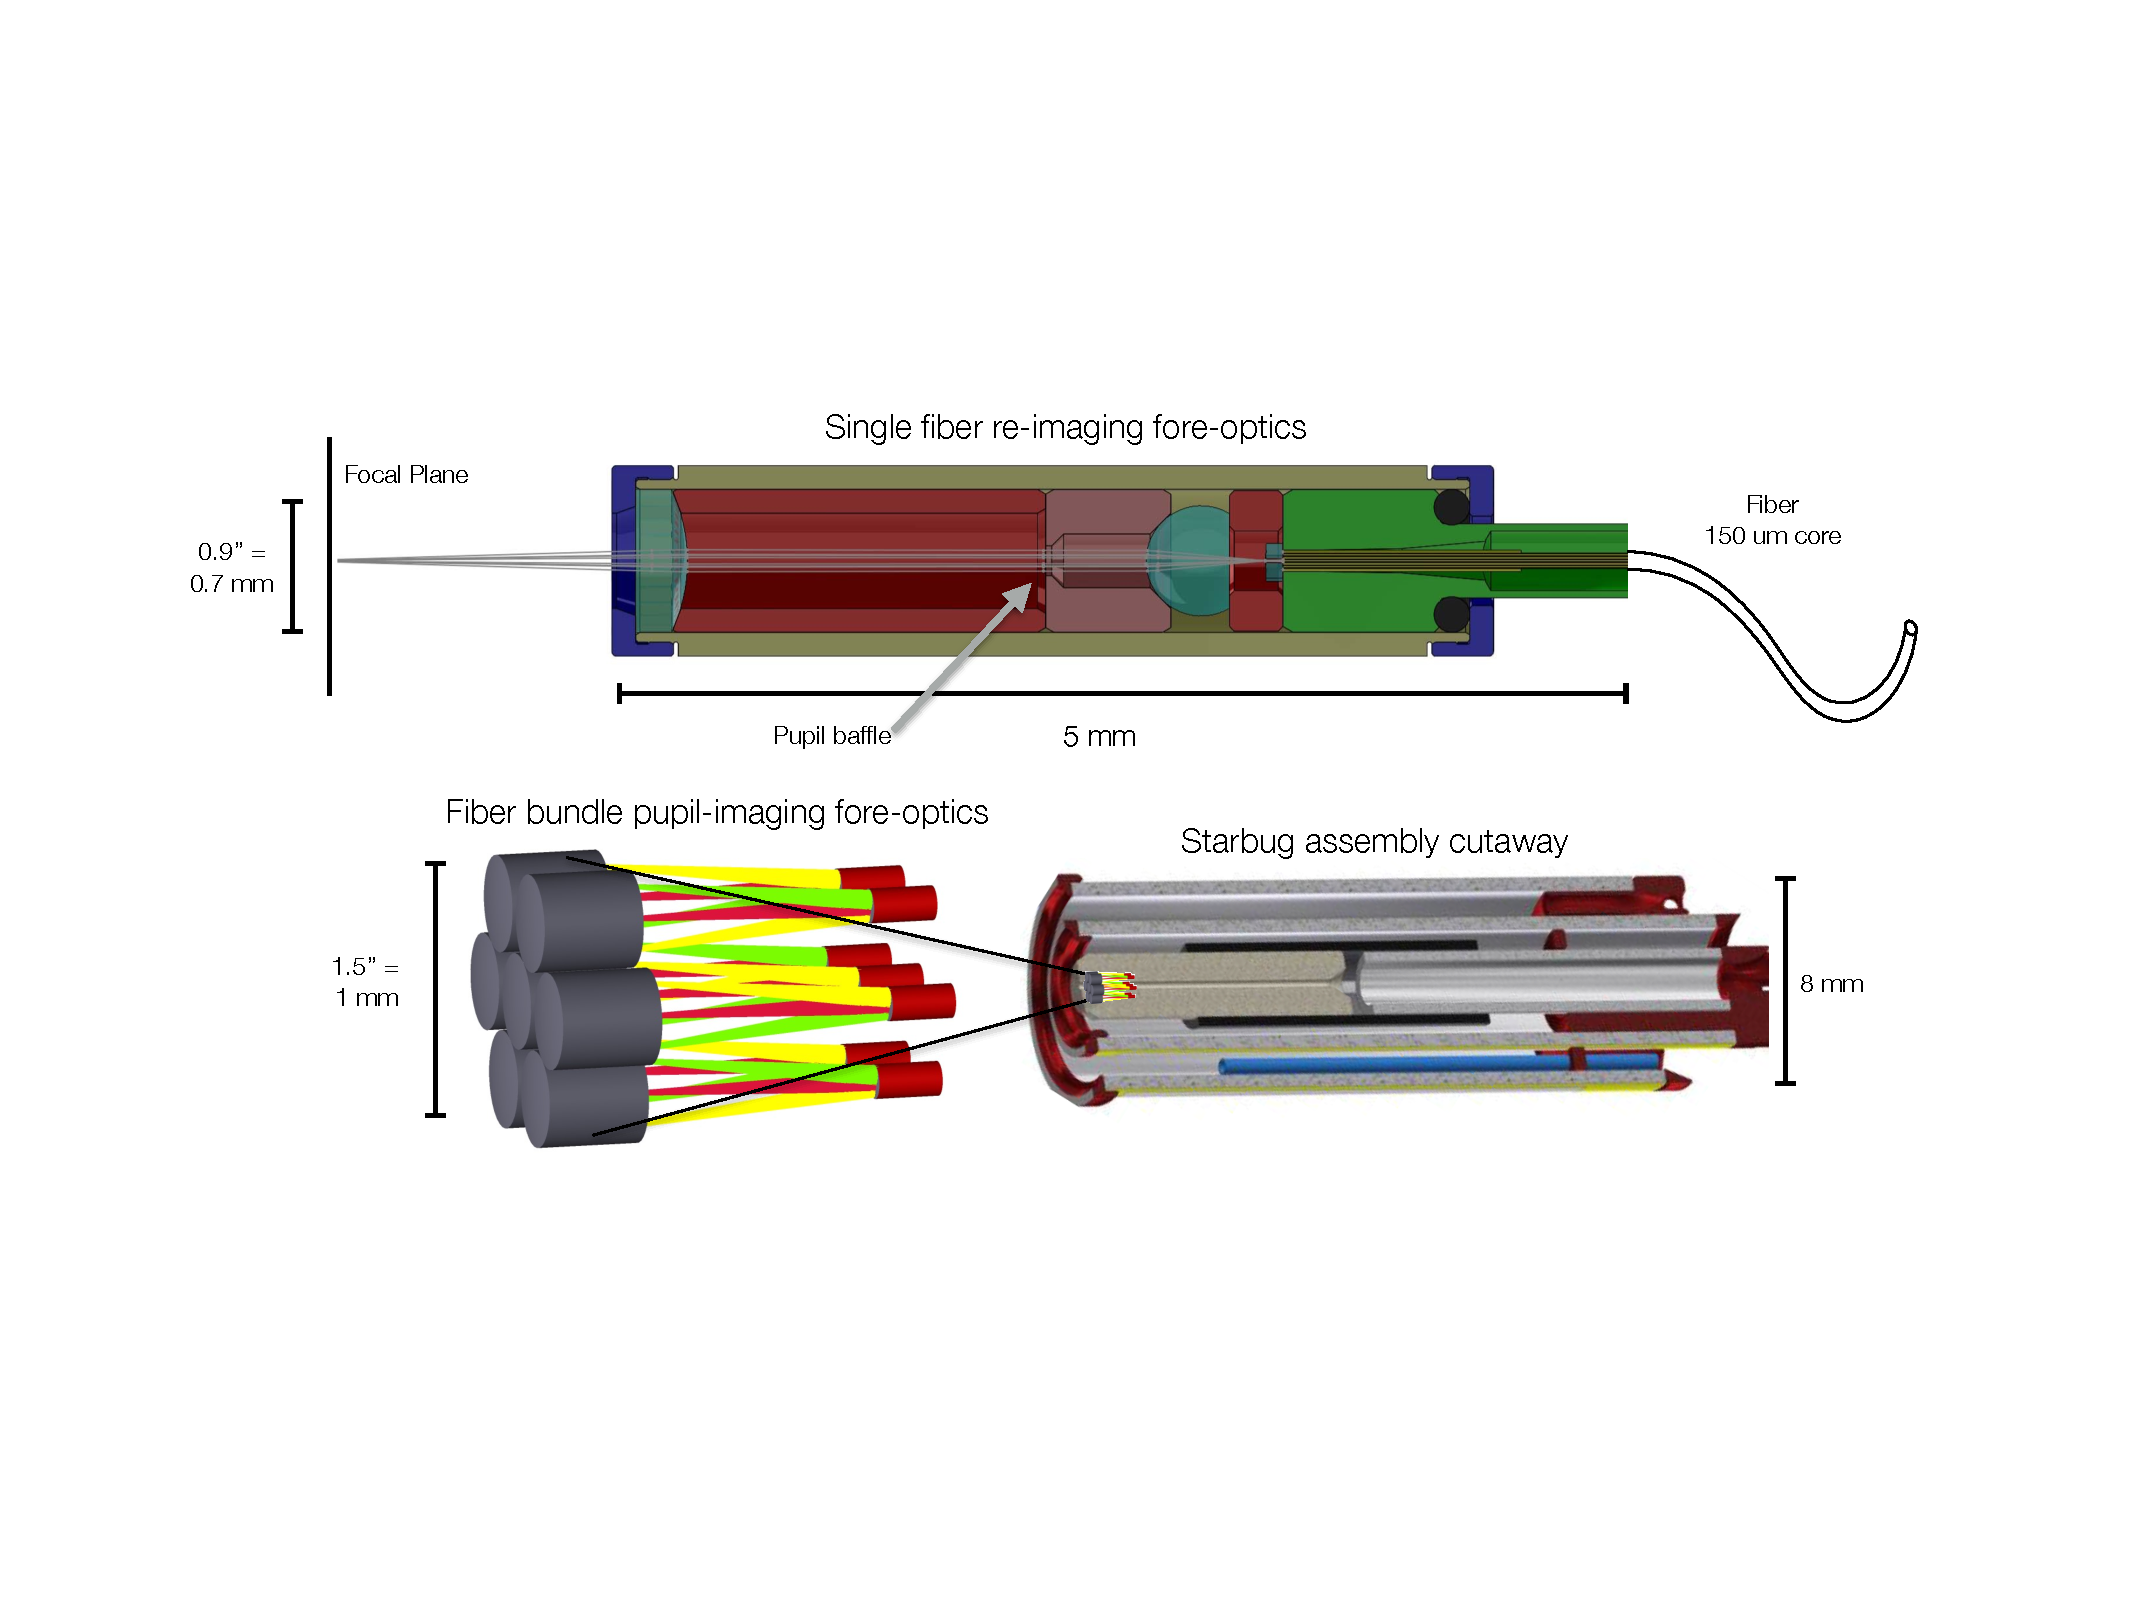
\includegraphics[width=0.9\textwidth]{figs/FOBOS_ForeOptics_v1.pdf}
\caption{\small {\it
Top}: Rendering of fiber coupling fore-optics and mechanical housing for a single fiber using focal-plane re-imaging.  Here the image at the focal plane is demagnified and re-imaged onto the fiber face.  The design allows for a pupil stop. {\it Bottom Left}: Optical layout for a 7-fiber microlens array.  As opposed to focal plane re-imaging, here the telescope pupil is imaged onto each fiber face.  {\it Bottom Right}: In either approach, the fore-optics are housed inside the much larger Starbug, a cutaway diagram of which is shown here. This on-going design work has been funded by the UCO \emph{FIDDLES} project.}
\label{fig:foreoptics}
\end{figure}
%%%%%%%%%%%%%%%%%%%%%%%%%%%%%%%%%%%%%%%%%%%%%%%%%%%%%%%%%%%%%%%%%%%%%%%%


\section{Recent and Ongoing Progress}
\label{sec:progress}

FOBOS development over the past year has focused on (1) engaging the
scientific and instrument-building communities in discussions about
the FOBOS design, particularly with regard to science cases and
instrument feasibility, (2) initial development of an instrument
simulator and exposure-time calculator, (3) advancing the
optomechanical designs of the focal-plane and ADC systems, (4)
consolidating development of Fiber-WFOS for TMT and repurposing much
of the design for FOBOS at Keck, (5) working with Keck instrument
scientists and engineers toward a practical integration plan, and (6)
developing a detailed project execution plan, schedule, and
short-term budget. Many of these activities were enabled by funds
provided in response to our previous white-paper submission.

Visits to Keck-user institutes have been particularly helpful in
building interest around the instrument and refining its
specifications. As of this writing, Bundy, MacDonald, and/or Westfall
have visited UCR (also joined by Michael Cooper from UCI), UCLA, Keck
observatory, LBNL, and UCSB. We plan to continue with visits to UCB, UCD, and CIT before the end of the year.

Feedback from the Keck community has emphasized the desire for very high multiplex, flexibility of the focal-plane
sampling, and sensitivity toward the UV. Although the capabilities of PFS are a common comparison for FOBOS, many of
the science goals now enumerated in Section 1 require target densities and/or wavelength coverage that PFS will not
provide. Another strong message from Keck users was the desire for deployable IFUs. Starbugs are attractive for this
reason becuase they make swapping focal-plane formats straightforward.

% Our
% initial concepts for these different focal-plane formats provided a
% secondary motivation for FOBOS's large pseudo-slit capacity: it can
% provide 15-100 smaller, freely deployable IFUs. Finally, Keck
% remains unique in its throughput toward the atmospheric limit. No
% other current or planned \comment{check this again} spectrograph for
% 10m-class telescopes provides sensitivity below $\sim$380nm,
% providing FOBOS with a unique capability among the landscape of
% forthcoming instrumentation.

% a large-format monolithic IFU and 

% yield a monolithic IFU with a FOV that is competitive with VLT/MUSE
% and can

\subsection{Fiber coupling and Fore-optics}
Another area of progress involves use of UCO funding to address risks in the
coupling of the microlens fore-optics to the fiber and the coupling
of the microlens entrance aperture to the Keck II focal plane (see Figure \ref{fig:foreoptics}).  This ``FIDDLES'' prototyping effort will test coupling performance in labs at UCO and LBL as well as on-sky at Lick and Keck Observatories.  Initial tests have begun and optomechanical designs were recently completed to enable hardware purchases.

% Finally, with the permission of the SSC, we proposed for
% instrument-design funds from the NSF via its new Mid-scale Research
% Infrastructure scheme. Although the proposal was ultimately
% unsuccessful, preparation of the proposal led to a ground swell of
% development in our project planning and science development, much of
% which is included in this submission.

\subsection{New technical expertise from DESI and PFS} Building on the FOBOS instrument team's experience with SDSS projects like BOSS, APOGEE, and MaNGA, we have recruited new expertise from DESI and PFS.  Claire Poppett at SSL/LBNL is DESI's Lead Fiber Scientist and has joined FOBOS to spearhead the fiber system and fore-optics development.  Tim Miller, also at SSL/LBNL, developed the DESI corrector's optical design and will take on the FOBOS ADC.  Renbin Yan, a scientist and instrument builder, has spent the last year at Princeton working with Jim Gunn on PFS-like calibration systems for future instruments.  Renbin was a heavy Keck observer for DEEP2 and will apply PFS knowledge on the calibration problem to Keck and FOBOS.

